\section{Introduction}
\red{Introductory examples from hospital, bank, government, etc.}

Distributed machine learning has been widely studied in order to handle exploding amount of data. It has also been reported that the volume and quality of data determines the upper bound of machine learning model performance. Privacy-preserving technique in distributed machine learning is one of the keys to encourage data sharing in distributed system. There are mainly two lines of works in privacy-preserving, encryption and differential privacy. Although encryption based methods have strong guarantee for data security, it has heavy computation overhead, which is not scalable. Differential privacy (DP) based methods are light weighted. Well designed DP algorithm can achieve good model performance under certain privacy guarantee. 

Most existing DP distributed machine learning works focus on data parallel scenario, where different subsets of the samples are distributed. To the best of our knowledge, few works are on the model parallel scenario, where different subset of the features are distributed. 

% \begin{figure}[t]
%     \centering
%     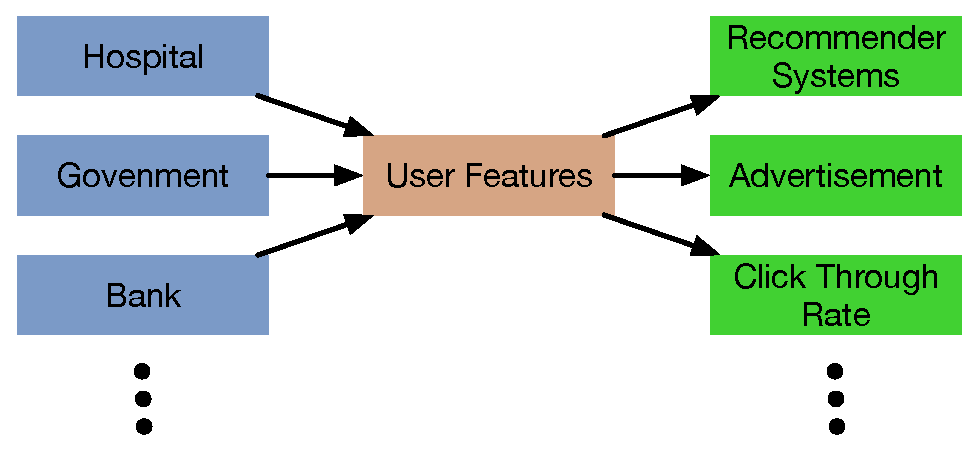
\includegraphics[width=3.2in]{figures/application.eps}
%     \caption{Applying Sensitive User Features to Other Applications}
%     \label{fig:application}
%     \vspace{-5mm}
% \end{figure}

We propose an efficient solution for the real application where features are distributed. In distributed machine learning system, convergence is a comprehension results of computation and communication. \red{In the case, ADMM sharing is a best suit since it is fast to converge in terms of epochs, which requires less privacy budget given certain accuracy.}

